
\documentclass[authordate, empirical,issue]{jote-new-article}

\usepackage{caption}

\usepackage{tabularx}

\usepackage{graphicx}

\usepackage{hyperref}


\usepackage{tikz}
\RequirePackage{xcolor}


\usepackage[backend=biber,style=apa]{biblatex}

\jotetitle{Medical expert endorsement fails to reduce vaccine hesitancy in U.K. residents}
\keywordsabstract{expert endorsement, Vaccine hesitancy, Nudging, Debunkning, COVID-19}
\abstracttext{In this report we outline the null findings of a pre-registered experiment on vaccine hesitancy in the United Kingdom. The experiment targeted vaccine misconceptions common among participants by presenting a correction to such claims endorsed by a group of medical experts. The experiment had the aim to increase vaccination intention and actual uptake during the 2021 COVID-19 vaccination campaign. Our results revealed that, contrary to a similar study conducted with Italian residents, our intervention was unsuccessful in changing participants’ attitudes and behaviour towards COVID-19 vaccines. The report concludes with a discussion of the potential reasons for these null findings.
 }
\runningauthor{Panizza et al.}
\jname{Journal of Trial \& Error}
\jyear{2023}
\paperdoi{10.36850/e15}
\paperreceived{March 20, 2023}
\author[1]{\mbox{Folco Panizza\orcid{0000-0001-5178-5926}}}
\affil[1]{Molecular Mind Laboratory, IMT School for Advanced Studies Lucca, Italy}
\corremail{\href{mailto:folco.panizza@imtlucca.it}{folco.panizza@imtlucca.it}}
\corraddress{Molecular Mind Laboratory}
\runningauthor{Panizza et al.}
\author[2]{\mbox{Piero Ronzani\orcid{0000-0002-8211-6028}}}
\affil[2]{International Security and Development Center, Berlin, Germany}
\author[3,4]{\mbox{Carlo Martini\orcid{0000-0001-9061-8020}}}
\affil[3]{Centre for Applied and Experimental Epistemology, Department of Philosophy, Vita-Salute
San Raffaele University, Milan, Italy.}
\author[5]{\mbox{Lucia Savadori\orcid{0000-0003-3957-3132}}}
\affil[4]{Centre for Philosophy of Social Science, De-
partment of Political and Economic Studies,
University of Helsinki, Helsinki, Finland.}
\author[3]{\mbox{Matteo Motterlini\orcid{0000-0002-4915-4524}}}
\affil[5]{Cognitive and Experimental Economics Laboratory, Department of Economics and Management, University of Trento, Trento, Italy}
\paperaccepted{July 6, 2023}
\paperpublished{September 7, 2023}
\paperpublisheddate{2023-09-07}
\jwebsite{https://journal.trialanderror.org}

\setcounter{page}{37}
\jissue{2}
\jvolume{4}
\jpages{37--48}
\specialissue{Scientific Failure and Uncertainty in the Health Domain}
\articletype{Special Issue - Empirical}

\addbibresource{bibliography.bib}

\usepackage{changepage}

\makeatletter
\let\@leftfloatplacement=\@floatplacement
\def\@rightfloatplacement{\global\@topnum=0
  % Textpage bit, global:
  \global\@toproom=\z@
  \global\@botnum=0
  \global\@botroom=\z@
  \global\@colnum=0
  % Floatpage bit, local:
  \@fpmin=\@colht}
\def\@floatplacement{\if@firstcolumn\@leftfloatplacement
  \else\@rightfloatplacement
  \fi}
\makeatother

\makeatletter
\patchcmd\@footnotetext{\footnotesize}{\footnotesize \predisplaypenalty=-100 }{}{\fail}
\makeatother
\begin{document}
\begin{frontmatter}
  \maketitle
  \begin{abstract}
    \printabstracttext
  \end{abstract}
\end{frontmatter}


\begin{tikzpicture}[remember picture, overlay]
    \node[align=left, text width=15cm, anchor=north west] 
    at ([xshift=4.7cm, yshift=-0.3cm]current page.north west) 
    {
        \noindent{\textbf{Correction notice}} \\
        Incorrect Special Issue Labeling (Article erroneously excluded): This article was previously not labeled as part of a special issue due to an error. This has now been corrected.\vspace{2pt}
        \noindent{{\color{joteorange}\rule{\linewidth}{1pt}}}
    };
\end{tikzpicture}




\lettrine{S}{cientists} and medical experts are among the professionals trusted the most (Skinner \& Clemence, 2022). Are they also the most suitable figures to convince the general public to get vaccinated? In a preregistered experiment, we tested whether expert endorsement increases the effectiveness of debunking messages about COVID-19 vaccines.



Recent literature underscores the significance of debunking in combating misinformation (Lewandowsky et al., 2020). Debunking involves presenting information that directly confronts the core misconception within a particular piece of false news. For instance, if an individual is averse to a vaccine due to a misplaced fear that it could cause autism in children (a case of false information), debunking would confront this belief directly by providing evidence from scientific studies that demonstrate no correlation between vaccination and autism in children. Corrections from experts can be an effective framing and communication strategy to steer people towards recommended policies (Bogliacino et al., 2021). We wanted to test the hypothesis that expert endorsement is an effective intervention to increase positive attitudes towards COVID-19 vaccines and intention to vaccinate.



The design of our debunking intervention was primarily guided by established dual process persuasion theories, such as the elaboration likelihood model (Petty \& Cacioppo, 1986), or the heuristic--systematic model (Chaiken, 1980). These theories propose that the credibility of the source, which includes perceived expertise, acts as a persuasive factor: individuals are more likely to be persuaded by a message originating from a credible source than from a less credible one (e.g., Heesacker et al., 1983). This is particularly true when the message is conveyed through a heuristic-peripheral route as opposed to a central-systematic one. Source expertise can significantly contribute to behavior change: debunking based on source credibility takes advantage of heuristic-peripheral processing in a setting (experimental survey) where respondents do not necessarily engage in central processing of information. For this reason, all debunking messages were endorsed by a source that is held in high regard by most of the general population, namely, medical experts and researchers. Interventions also draw upon the extensive body of literature emphasizing the role of social norms in changing human behavior (Reynolds, 2019). From this perspective, individuals are perceived as social beings who endeavor to maintain their place in groups composed of individuals they respect, admire, and identify with. In this sense, the opinion of experts influences certain behaviors because experts are seen as a generally respected group of individuals who possess relevant knowledge.



We sought to apply this framework by framing expert endorsement as a social norm: specifically, expert endorsement was presented as a majority consensus of qualified and trusted experts (van der Linden, 2021).

\begin{takeHomeMessage}

  An intervention based on medical expert endorsement may not have been successful in improving vaccination intention and actual uptake during the 2021 COVID-19 immunisation campaign in the United Kingdom. The message campaign that was specifically built on experts' advice did not change participants' views or behaviour concerning COVID-19 vaccinations. Further research is needed to determine why a similar intervention succeeded in an Italian sample but not among respondents in the United Kingdom.

\end{takeHomeMessage}

Finally, the interventions were specifically tailored to the sample: messages sent to participants targeted their personal concerns about COVID-19 vaccination as expressed in a pre-screening survey. This ensured that the messages were relevant to respondents and increased the likelihood that they would attend the messages.



We monitored a sample of 2,247 people in the United Kingdom through a longitudinal study along the salient phases of the vaccination campaign. Participants in the “expert endorsement” treatment received a series of messages targeting concerns expressed by participants themselves about COVID-19 vaccines. Messages were endorsed by a majority of medical experts consulted on these concerns. In order to minimise demand effects, we collected participants' responses about ten days after the previous debunking message. To test the effectiveness of the intervention, we also monitored beliefs, intentions, and vaccination behaviour of a control group. Contrary to pre-registered hypotheses, vaccination turnout did not increase in the experimental sample compared to control, nor did participants express a higher intention to vaccinate, or more positive beliefs about the protective benefits of vaccines. This lack of evidence contrasts with the results of a similar experiment conducted among Italian residents, (Ronzani et al., 2022) in which the intervention supported by experts was compared with the same intervention supported by a generic group of survey respondents. In the Italian experiment, vaccination intentions and beliefs about the protective benefits of vaccines increased in the expert treatment compared to the non-expert version. Conversely, the same expert intervention had no effect on these measures in the sample of UK participants.\footnote{ For more context about the experimental literature, please consult the twin publication of this report:\href{https://doi.org/10.1016/j.vaccine.2022.06.031}{doi.org/10.1016/j.vaccine.2022.06.031.}}



\section{Methods}



Participants were first recruited from the online platform Prolific through a screening survey at the beginning of the vaccination campaign (\emph{N }= 2598). Collection started on the 12th of January 2021. The goal of this survey was to collect preliminary information about participants' demographics, their initial willingness to receive a vaccine (vaccination intention) and, for vaccine hesitants, their main concern keeping them from getting vaccinated. Questions were adapted from previous Ipsos surveys (Boyon \& Silverstein, 2021). Although we did not aim to collect a sample that was representative of the general U.K. population nor did we have any specific demographics predictions, we tried as much as possible to balance the composition of the sample in terms of education. Educational stratification was introduced to match national rates as closely as possible and to avoid biasing the results by, for example, oversampling the educated. Our sample was thus recruited based on quotas defined by the most recent data available about the level of education of U.K. residents (Office for
National Statistics, 2019)\footnote{We decided to exclude the 'other education' category from the survey since it was not possible to match this category with data available for participants on Prolific. It may in fact have been the case that foreign degrees that the Office for National Statistics considers as 'other education' \href{https://www.ukdataservice.ac.uk/media/262853/discover_sqb_education_schneider.pdf}{(www.ukdataservice.ac.ukmedia262853discover\_sqb\_education\_schneider.pdf)} were instead reported by the participants as equivalent to UK degrees, thus producing a mismatch in classification. We thus decided to keep the proportions for the other education levels while removing this category.\par We did not carry out any analysis including education as we controlled for this variable through sampling and had no pre-registered hypothesis related to it.}.

\begin{table}
  \begin{fullwidth}
    \caption{Number of participants and retention rate for each wave of the study.}
    \begin{tabularx}{\linewidth}{@{} X X X @{}}
                                           & \multicolumn{2}{c}{\hspace*{-3em}\textbf{Group}}                         \\
      \textbf{Wave}                        & \textbf{Control}                                 & \textbf{Experimental} \\
      \hline \textbf{1}: \emph{April 6–15} & 1063 (100\%)                                     & 1057 (100\%)          \\

      \textbf{2}: \emph{April 16–25}       & 1037 (97.6\%)                                    & 1051 (99.4\%)         \\

      \textbf{3}: \emph{April 26–May 5}    & 1038 (97.7\%)                                    & 1046 (99.0\%)         \\

      \textbf{4}: \emph{May 6–15}          & 1020 (96.0\%)                                    & 1004 (95.0\%)         \\

      \textbf{5}: \emph{May 16–25}         & 983 (92.5\%)                                     & 996 (94.2\%)          \\

      \textbf{6}: \emph{May 26–June 4}     & 957 (90.0\%)                                     & 977 (92.4\%)          \\

      \textbf{7}: \emph{June 5–14}         & 985 (92.7\%)                                     & 1010 (95.6\%)         \\
    \end{tabularx}
  \end{fullwidth}
\end{table}

The size of the sample was determined based on the number of available participants in the least represented education category on prolific ("no formal education"). To be eligible, participants must not have received the vaccine at the time of the survey. We tried to collect as many participants as possible given the constraints of the recruiting platform, the goal of having a fairly representative national sample in terms of education level, and the progress of vaccination campaign. We recruited an initial sample of 2598 U.K. residents based on these criteria. Participants were then randomised into an experimental group and a control group, while keeping the proportion of vaccine hesitancy and education balanced between the two groups. 59 participants were excluded in the process because they were missing demographic information (employment data) or because they reported being already vaccinated. We were thus left with a sample of 2539 eligible participants. The Research Ethics Committee of the University of Trento approved the study (protocol no. 2021-001) and subjects provided written informed consent prior to their inclusion. All participants were paid for their time.



The experiment was organised in seven consecutive waves spanning 10 days each. Data collection for the experiment started on the 6th of April 2021. Participants had 10 days to respond to the survey, after which data collection for that wave was closed and a new wave started at the eleventh day. All surveys were scheduled to start at around the same time (14.00 GMT). The longitudinal design of the study included six interventions and a final survey, for a total of seven waves. Although analyses were conducted on participants having completed all seven waves, we also conducted robustness analyses on participants who completed fewer waves. For this reason, we allowed participants to respond to surveys even if they missed previous waves, including the first one\footnote{ This fact is reflected in the attrition rate of Table 1, which can also be negative (see the increase of participants in the control treatment between wave 2 and wave 3). Robustness analyses include participants who completed fewer waves, with and without excluding participants re-entering the experiment. These analyses yield the same statistical results as in the main text (see Supplementary Analyses).}. We excluded one participant that moved their residence outside the United Kingdom during data collection. We also excluded one more participant who was missing educational information. We also excluded single responses under specific circumstances. Some participants responded more than once in the same wave, hence we decided to keep their first response only, as the subsequent ones might have been influenced by previous responses. Furthermore, we excluded participant responses from specific analyses in case their responses were not logically plausible. For instance, we excluded data from participants reverting their vaccination status between waves (from "vaccinated" to "not vaccinated") for analyses concerning vaccination behaviour. The final sample size of participants included in any one analysis was \emph{N }= 1119 for the control group, and \emph{N }= 1128 for the expert endorsement group (total \emph{N }= 2247). Table 1 represents the number of participants in each group after exclusion criteria were applied, and the retention rate compared to the initial sample (Supplementary Tables A.3 and A.4 show the same data broken down by level of education; Supplementary Table A.5 shows instead the proportion of participants in each treatment divided by how many waves were completed).





\begin{figure*}[bh!]
  \begin{fullwidth}
    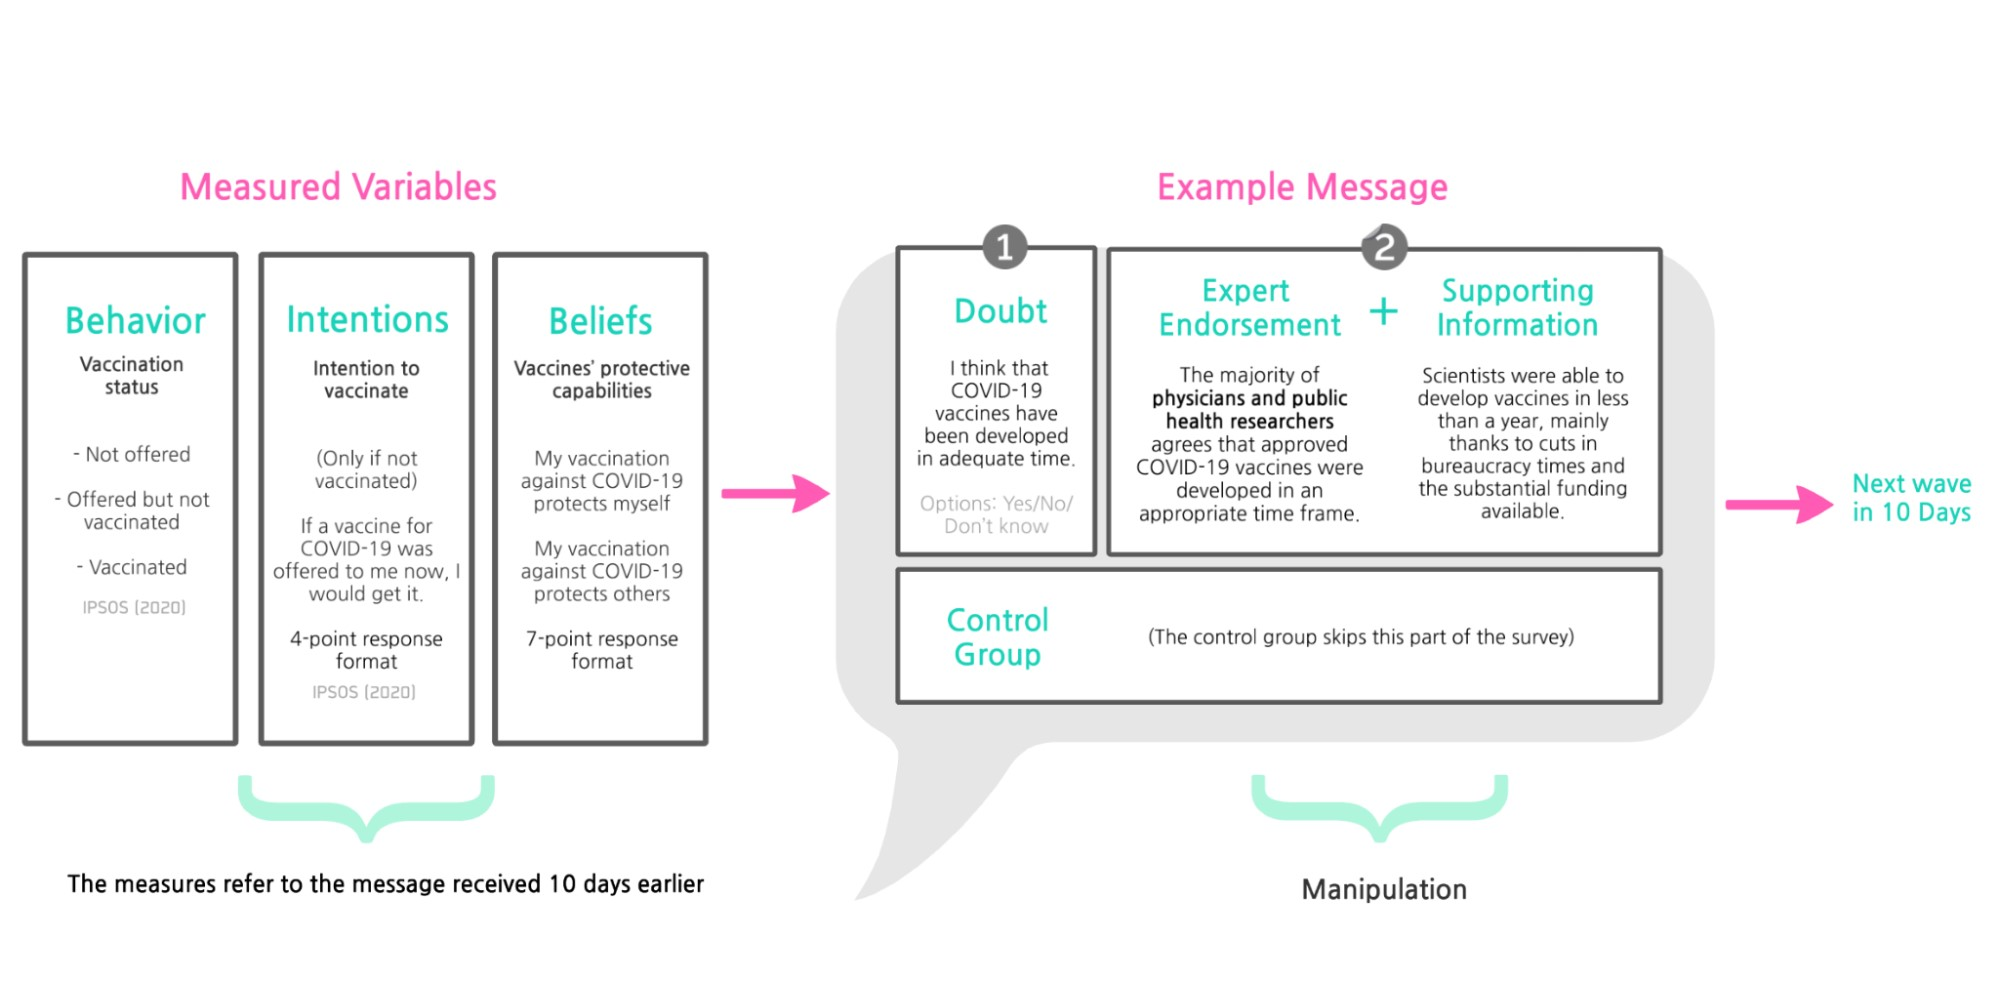
\includegraphics[width=\linewidth]{media/image1.jpg}

    \caption{Flow-chart of one exemplary wave. The wave starts with the recording of vaccination behaviour, intentions, and beliefs (used as outcomes of the previous message intervention). The recording of the measures of interest are followed in the expert treatment group by the debunking message endorsed by experts.}

    \label{fig:rId9}

  \end{fullwidth}
\end{figure*}




\subsection{Experimental design}

Participants responded to up to seven waves. All waves measured our variables of interest (vaccine behaviour, intention and beliefs), and all waves except the last one included a message intervention. In each wave, participants were first asked about their vaccination status (not offered; offered but not vaccinated; vaccinated), their intention to vaccinate (if not vaccinated: "If a vaccine for COVID-19 was offered to me now, I would get it."; four-point response format from "strongly disagree" to "strongly agree"), and their beliefs about vaccines' protective capabilities for themselves and others (two questions: "My vaccination against COVID-19 protects [myself/others]"; seven-point response format from "completely disagree" to "completely agree"). Questions about vaccination status and intention were adapted from previous Ipsos surveys (Boyon \& Silverstein, 2021) to keep results comparable.



After responding to the initial questions, participants observed the message interventions (example in Figure 1). One message was created for each wave, and all messages were built around participants' initial concerns about vaccines, which we collected in the preliminary survey. For example, one of the most common concerns was the fact that vaccines had been developed too quickly; the correlated informative intervention stressed the fact that SARS-CoV-2 vaccines' fast development was possible by cutting most bureaucratic times.











For each wave, participants in the expert endorsement treatment received one message intervention that included three parts: Participants were first asked their opinion about the concern targeted in that wave (e.g., "I think one should be vaccinated even if there may be side effects."; options: Yes/No/Don't know). After expressing their opinion, participants in the expert endorsement group observed a message in response to the concern. This response was based on the evaluation of doctors and COVID-19 researchers who were shown participants' concerns (see Supplementary Material Expert Survey). The response was phrased as follows: "In the January survey in which you participated, we collected some concerns about vaccination against COVID-19. We recently conducted a second survey among doctors and researchers: The majority of experts agrees that [message]"\footnote{ The message emphasises that these are not general statistics, but rather data that have been collected by the experimenters from a specific sample of medical researchers. This notwithstanding, we did not include the names or affiliations of the experts interviewed, as this information may have influenced participants' responses more than the message itself, and may have reduced the generalizability of the findings, for example because the name of the expert or institution may have polarised responses.}. The third and last part of the intervention was a text providing support for the endorsement message. Participants in the control treatment did not observe the endorsement nor the message. Messages were based on material from leading health institutions (U.S. Centers for Disease Control and Prevention, European Medicines Agency, U.K. National Health Service). Note that message interventions appeared \emph{after }we collected participants' vaccination status, intention, and beliefs. This ensured that participants' answers were not distorted by any potential demand effect. We expected instead that our messages affected responses in the subsequent wave. The complete list of interventions is available at \href{https://osf.io/m8cr6/}{osf.io/m8cr6.}



The last wave did not include a message, but a series of control questions. Participants answered further questions regarding the COVID-19 pandemic and vaccination campaign. Questions included whether participants completed the vaccination cycle and if they contracted COVID-19 in the previous three months (Yes/No questions), whether they would recommend a vaccine to friends and relatives (five-point response format from "completely disagree" to "completely agree"), and a scale measuring coronavirus risk perception (Savadori \& Lauriola, 2021). Participants were also asked their main source of information about COVID-19 (multiple choice question) and their trust in the national government, scientists, and pharmaceutical companies ("not at all"/"not much"/"some"/"a lot"/"don't know"; questions adapted from the 2018 Wellcome Global Monitor, 2018). Lastly, participants completed a survey with a series of scales, including the short-form version of the cultural worldview scale (Kahan, 2021), and the Conspiracy Ideation Trait scale (Bode \& Vraga, 2018).



\subsection{Analyses}



Analyses were conducted in R (R Core Team, 2018) using the multgee (Touloumis et al., 2013) package package. To test for changes in vaccination uptake we used a Chi squared test comparing the proportion of vaccinated participants between the two experimental treatments. We included only those participants who were offered a dose of vaccine by the end of the experiment (\emph{N }= 812). To capture changes in vaccination intention, we included only participants who were not yet offered a dose of vaccine at the end of data collection (\emph{N }= 280). We adopted a repeated measure, ordinal logistic regression for the analysis, including survey wave, experimental group, and their interaction as predictor variables, and participant id as random factor. We interpret the interaction between wave and group as our measure of difference in difference, whereas we consider the non-interaction variables as control measures. Although our analyses focused on participants who completed all waves of the experiment, we include also robustness tests including participants who dropped out before the conclusion of the study and therefore observed fewer messages. Finally, changes in beliefs about vaccines were tested on all participants who completed the study (\emph{N }= 1599). We adopted the same statistical test as for vaccination intentions, repeated for both our belief questions (protection for self, protection for others). We adopted the 5\% significance level to test against the null hypotheses. Post-hoc tests and multiple analyses were corrected for multiple comparisons using a Benjamini-Hochberg procedure. Square brackets indicate family-wise corrected 95\% confidence intervals.



\section{Results}



\subsection{Vaccination uptake}



As part of our pre-registered analyses, we selected all those participants who reported that they were offered a dose of vaccine between the beginning and the end of the experiment. We tested whether having been assigned to the expert endorsement treatment increased self-reported vaccination uptake compared to control. With the percentage of vaccinated in the last wave being 61.7\% in the expert endorsement treatment and 59.6\% in the control group, we did not find a significant difference in the percentage of individuals reporting having been vaccinated (\emph{χ}\textsuperscript{2}(1) = 0.280, \emph{p }= 0.597, \emph{BF}\textsubscript{10 }= 0.103).



\subsection{Intention to vaccinate}



Participants' propensity to vaccinate was positively but not significantly affected by expert endorsement, as measured as a difference in difference between experimental and control group across waves (interaction term wave × treatment: \emph{β }= .008[-.046, .061], \emph{z }= 0.279, \emph{p }= .780). Instead, vaccination intention increased significantly with time in both groups (\emph{β }= .042[.009, .076], \emph{z }= 2.501, \emph{p }= .012). Note that there were no significant differences in intention to vaccinate between the two groups at the beginning of the experiment (\emph{β }= .123[-.371, .617], \emph{z }= 0.487, \emph{p }= .626).



Results reported above include only participants who completed the experiment. We additionally explored how many messages are sufficient to observe a significant effect of expert endorsement on intention\footnote{ Interpretation of these analyses is valid if there are no confounding factors affecting how many waves participants completed before dropping out. In other words, whether or not taking part in some waves of the study should not be dictated by endogenous factors. A potential confound is that only participants who were strongly motivated completed multiple consecutive waves. For this reason, we allowed participants to re-enter the experiment even after missing waves. We repeated the analysis by including these data points and found comparable results to the ones reported in the main text (Supplementary Table Appendix A.4).}. Table 2 reports results including different subsets of the sample: the first row includes only participants who read all 6 messages (results above), whereas the last one includes participants who read at least 1 message or more. Regardless of the messages exposed, effect of time is significant and robust, whereas the effect of the intervention remains non-significant.










\begin{table*}
  \begin{fullwidth}
    \caption{Vaccination intention as a function of the number of consecutive messages read.}
    \resizebox{\textwidth}{!}{
      \tiny
      \begin{tabular}{@{} l l l l l l l l l l l @{}}
        \hline                                            & \textbf{N} & \multicolumn{2}{l}{\textbf{Expert endorsement}} &                       &
        \multicolumn{2}{l}{\textbf{Control group}}        &            &
        \multicolumn{2}{l}{\textbf{Baseline differences}} &                                                                                                                                                                                 \\

        Messages                                          &            & \emph{β}                                        & z                     & \emph{p} & \emph{β}            & z     & \emph{p} &
        \emph{β}                                          & z          & \emph{p}                                                                                                                                                           \\
        6                                                 & 280        & 0.008 [-0.046,0.061]                            & 0.279                 & 0.780    & 0.042 [0.009,0.076] & 2.501 & 0.012*   & 0.123 [-0.371,0.617] & 0.487 & 0.626 \\
        \textbf{5+}                                       & 295        & 0.009 [-0.040,0.059]                            & 0.373                 & 0.709    &
        0.043 [0.012,0.074]                               & 2.745      & 0.006**                                         & 0.096 [-0.381,0.573]  & 0.395    &
        0.693                                                                                                                                                                                                                               \\

        \textbf{4+}                                       & 323        & 0.009 [-0.040,0.057]                            & 0.347                 & 0.729    &
        0.043 [0.012,0.074]                               & 2.752      & 0.006**                                         & 0.044 [-0.407,0.496]  & 0.192    &
        0.847                                                                                                                                                                                                                               \\

        \textbf{3+}                                       & 355        & 0.007 [-0.042,0.056]                            & 0.281                 & 0.778    &
        0.045 [0.013,0.077]                               & 2.746      & 0.006**                                         & -0.013 [-0.449,0.424] & -0.056   &
        0.955                                                                                                                                                                                                                               \\

        \textbf{2+}                                       & 386        & 0.004 [-0.045,0.053]                            & 0.168                 & 0.867    &
        0.044 [0.011,0.076]                               & 2.642      & 0.008**                                         & -0.028 [-0.450,0.395] & -0.129   &
        0.897                                                                                                                                                                                                                               \\

        \textbf{1+}                                       & 416        & 0.006 [-0.043,0.055]                            & 0.227                 & 0.820    &
        0.042 [0.010,0.074]                               & 2.574      & 0.010*                                          & -0.010 [-0.419,0.398] & -0.050   &
        0.960                                                                                                                                                                                                                               \\
      \end{tabular}}
  \end{fullwidth}
\end{table*}









\subsection{Beliefs about vaccines}



Regression analyses for vaccine beliefs did not reveal any significant effect of expert endorsement: after the experiment, participants in the experimental group reported around the same beliefs about the protectiveness of vaccines compared to the control group. This was true for both questions, protection to self (\emph{β }= -.010[-.031, .012], \emph{z }= -0.873, \emph{p }= .383) and protection for others (\emph{β }= .009[-.013, .031], \emph{z }= 0.816, \emph{p }= .414). Our control variables suggest that beliefs about the protection for others did increase over time in both groups (\emph{β }= .030[.015, .044], \emph{z }= 4.063, \emph{p < }.001), but this increase was not significant for beliefs about the protection for self (\emph{β }= .007[-.008, .022], \emph{z }= 0.958, \emph{p }= .338). Our tests also indicate that beliefs did not significantly differ at the beginning of the experiment (self: \emph{β }= .066[-.108, .240], \emph{z }= 0.744, \emph{p }= .457; others: \emph{β }= .025[-.146, .195], \emph{z }= 0.284, \emph{p }= .776). As a final robustness check, we test whether the role of the expert is also significant when including dropped-out participants. These tests confirm the non-significant effect of the intervention (Supplementary Tables in Appendix A.5).



\section{Discussion}



This study aimed at testing the effectiveness of an intervention meant to promote positive beliefs about vaccines and to increase vaccination intention and uptake in a sample of U.K. residents. The intervention consisted of providing participants with pieces of information about the COVID-19 vaccine that addressed their reasons for being hesitant in vaccinating (debunking information). Concerns were expressed by the participants themselves in a preliminary survey, and response messages were vetted by a team of medical experts and researchers. Informative text snippets were provided to the same individuals in seven different waves, 10 days apart from each other. To test the effect of the intervention, we also monitored vaccine beliefs, intentions and behaviour in a control group that did not receive any of the messages.



Results show that expert endorsement did not have a significant effect on vaccination uptake, nor on vaccination intentions or beliefs about the protectiveness of COVID-19 vaccines. Our pre-registered analyses yielded null results, thus not supporting the original predictions. These results come in contrast to findings from an Italian sample who underwent a similar intervention (Ronzani et al., 2022). One design deviation from the current study was that the control group also received the intervention messages, but these were endorsed by a generic "majority of respondents" (thus not specifying the qualifications of the experts). In this study, we found that while vaccination uptake did not significantly increase, both vaccination intentions and beliefs were more positive after the intervention.

\begin{originalPurpose}



  The study's original aim was to test whether expert endorsement improves the impact of debunking messages about COVID-19 vaccines in the United Kingdom. The intervention targeted common vaccine misunderstandings held by participants by presenting a correction to such beliefs backed up by a panel of medical professionals. The ultimate goal of the study was to increase vaccination intention and actual uptake during the 2021 COVID-19 immunization campaign.

\end{originalPurpose}

What factors could explain the differences between these two studies? Below are a number of hypotheses that could in part explain this gap. Firstly, data from the two studies were collected in parallel, but the phases of the vaccination campaigns in the two countries did not coincide. As a reference, half of the eligible Italian population was administered at least a dose of the vaccine by the first week of July 2021, after the start of the experiment. In the UK, this event occurred around mid-March, much earlier than in Italy and before the start of the experiment. Not only was the timing of the campaign different, but also the policies discussed, such as the European COVID certificate, as well as the results of negotiations with vaccine companies. Indeed, since Brexit, many key negotiations and policies have been conducted separately for the UK and EU countries, which in turn may have influenced the topics covered in the media and public opinion. Distinct conditions could partly explain the non-significant results in the United Kingdom: a higher rate of vaccinations at the beginning of the experiment reduced the sample size available for analyses about vaccination intention: indeed, of those who completed all experimental waves, only 12 participants in the expert endorsement treatment initially reported that they were unwilling to be vaccinated when possible, compared to 20 in the control treatment. This may have contributed to a ceiling effect in the effectiveness of the intervention. However, a small number of vaccine hesitant participants would still not explain the non-significant difference between the two groups with regard to beliefs about the protectiveness of the vaccine. In fact, the number of sceptics was considerably larger and more balanced among the treatments. In this respect, other elements may have contributed to the non-significant effect of our intervention, such as a different responsiveness to our messages. For example, exploratory analyses (Appendix A.3) suggest that the debunking message displayed in the first wave (about the time frame for vaccine development) was more likely to address concerns expressed by the Italian sample than by UK respondents, potentially making our intervention less effective. These and other differences may be the result of an effective communication campaign by the U.K. government or the National Healthcare System. Indeed, our data show that over the course of the experiment there was a significant increase in vaccination intentions and beliefs about the protective capabilities of vaccines towards others. Although there is no significant increase in the belief that vaccines can protect oneself, the numbers related to this belief were already quite high at the beginning of the experiment. Additional differences might have contributed to the observed results, such as socio-cultural differences (e.g., the entrenchment and spread of no-vax movements in the two countries, trust in the healthcare system, etc.), the level of education in the two samples (stratified in the U.K. sample, unstratified and generally high in the Italian sample), as well as events of national resonance, such as the suspension of the Astra-Zeneca vaccine in Italy. These various discrepancies make comparing the two data sets an arduous task, despite the similarity of the experimental designs.



One more explanation to our non-significant results that seems unlikely is experimenter demand effect (Zizzo, 2009). This effect predicts that participants report differently from their real intentions because they want to fulfil the experimenter's presumed expectations. Participants in the control treatment may have conveniently concealed the offer of vaccination in order not to report their refusal of the vaccine, or they may have declared their intention to vaccinate while remaining, in reality, hesitant. We remain unconvinced by this explanation, as the control treatment did not cue any kind of intention on the part of the experimenters, thus making it unlikely that the participants unambiguously changed their behaviour towards a more pro-vaccine attitude. One final explanation is that the intervention that we designed might simply not be effective in certain populations (Bryan et al., 2021). As we note in Ronzani et al. (2022) The cultural characteristics of Italy make it peculiar in more than one way, and thus we may observe a certain degree of heterogeneity between populations more or less similar to this specific country. Further replications of the current design in different regions of the world will be needed to verify this explanation.




\section{Conclusions}



In this longitudinal study that followed a group of U.K. residents over the course of several months, we recorded their concerns, beliefs, attitudes and choices about vaccines. By offering information endorsed by experts addressing the main doubts raised by hesitant people (debunking), we attempted to increase participants' intention to vaccinate and, consequently, vaccination uptake. Our results, however, reveal that our intervention was ineffective in achieving these results, or in changing participants' beliefs about the protectiveness of vaccines. Further research is needed to understand why a similar intervention has worked in an Italian context but not among residents of the United Kingdom.



\section{Acknowledgments}



We would like to thank Sergiu Burlacu and Austeja Kazemekaityte for advice on the design and Maria Almudena Claassen for her magic plot advice. We would also thank the attendee of SPUDUM 2021, TIBER Symposium 2021, and INEM 2021.


\section{Funding}
This project has received funding from the European Union's Horizon 2020 research and innovation programme under grant agreement No 870883. The information and opinions are those of the authors and do not necessarily reflect the opinion of the European Commission.

\section{References}

Bode, L., \& Vraga, E. K. (2018). See something, say something: Correction of global health misinformation on social media. \emph{Health Communication, 33}(9), 1131–40. \url{https://doi.org/10.1080/10410236.2017.1331312}

Bogliacino, F., Charris, R., Gómez, C., Montealegre, F., \& Codagnone, C. (2021). Expert endorsement and the legitimacy of public policy. Evidence from Covid19 mitigation strategies. \emph{Journal of Risk Research, 24}(3-4), 394–415. \url{https://doi.org/10.31235/osf.io/zbqjd}

Boyon, N., \& Silverstein, K. (2021). Global attitudes: COVID-19 vaccines. \emph{Ipsos}. \url{https://www.ipsos.com/en-ro/global-attitudes-covid-19-vaccine-january-2021}

Bryan, C. J., Tipton, E., \& Yeager, D. S. (2021). Behavioural science is unlikely to change the world without a heterogeneity revolution. \emph{Nature Human Behaviour, 5}(8), 980–9. \url{https://doi.org/10.1038/s41562-021-01143-3}

Chaiken, S. (1980). Heuristic versus systematic information processing and the use of source versus message cues in persuasion. \emph{Journal of Personality and Social Psychology, 39}(5), 752–766. \url{https://doi.org/10.1037/0022-3514.39.5.752}

Heesacker, M., Petty, R. E., \& Cacioppo, J. T. (1983). Field dependence and attitude change: Source credibility can alter persuasion by affecting message-relevant thinking. \emph{Journal of Personality, 51}(4), 653–66. \url{https://doi.org/10.1111/j.1467-6494.1983.tb00872.x}

Kahan, D. M. (2021). Cultural cognition as a conception of the cultural theory of risk. In S. Roeser, R. Hillerbrand, P. Sandin, \& M. Peterson (Eds.), \emph{Handbook of risk theory: Epistemology, decision theory, ethics, and social implications of risk}. Springer Dordrecht. \url{https://doi.org/10.1007/978-94-007-1433-5\_1}

Lewandowsky, S., Cook, J., Ecker, U. K. H., Albarracín, D., Amazeen, M. A., Kendeou, P., Lombardi, D., Newman, E. J., Pennycook, G., Porter, E., Rand, D. G., N., R. D., J., R., Roozenbeek, J., Schmid, P., Seifert, C. M., Sinatra, G. M., Swire-Thompson, B., van der Linden, S., \& Vraga, E. K. (2020). Databrary. \url{https://doi.org/10.17910/b7.1182}

Office for National Statistics. (2019). Highest level of qualification achieved by people living in UK regions. \url{https://www.ons.gov.uk/peoplepopulationandcommunity/educationandchildcare/adhocs/10516highestlevelofqualificationachievedbypeoplelivinginukregions2010to2018}

Petty, R. E., \& Cacioppo, J. T. (1986). \emph{Communication and persuasion: Central and peripheral routes to
attitude change}. Springer. \url{https://doi.org/10.1007/978-1-4612-4964-1}

R Core Team. (2018). \emph{R: A language and environment for statistical computing}. R Foundation for Statistical Computing. \url{https://www.R-project.org/}

Reynolds, K. J. (2019). Social norms and how they impact behaviour. \emph{Nature Human Behaviour, 3}(1), 14–15. \url{https://doi.org/10.1038/s41562-018-0498-x}

Ronzani, P., Panizza, F., Martini, C., Savadori, L., \& Motterlini, M. (2022). Countering vaccine hesitancy through medical expert endorsement. \emph{Vaccine, 40}(32), 4635–43.

Savadori, L., \& Lauriola, M. (2021). Risk perception and protective behaviors during the rise of the COVID-19 outbreak in italy. \emph{Frontiers in Psychology, 11, Article 577331}.

Skinner, G., \& Clemence, M. (2022). Ipsos veracity index 2022. \emph{Ipsos}. \url{https://www.ipsos.}

Touloumis, A., Agresti, A., \& Kateri, M. (2013). GEE for multinomial responses using a local odds ratios parameterization. \emph{Biometrics, 69}(3), 633–40. \url{https://doi.org/10.1016/j.vaccine.2022.06.031}

van der Linden, S. (2021). The gateway belief model (GBM): A review and research agenda for communicating the scientific consensus on climate change. \emph{Current Opinion in Psychology, 42}, 7–12. \url{https://doi.org/10.1016/j.copsyc.2021.02.005}

Zizzo, D. J. (2009). Experimenter demand effects in economic experiments. \emph{Experimental Economics, 13}(1), 75–98. \url{https://doi.org/10.2139/ssrn.1163863}



\clearpage
\onecolumn
\appendix




\renewcommand\thefigure{A.\arabic{figure}}
\renewcommand\thetable{A.\arabic{table}}

\section{Appendix A. Materials and Methods}



\subsection{Appendix A.1. Waves completed}


\begin{table}[h!]
  \begin{fullwidth}
    \caption{Number of participants and retention rate for each wave of the study, by level of education, Control group.}
    \resizebox{\textwidth}{!}{
      \tiny
      \begin{tabular}{@{} l l l l l l l l l @{}}
        \hline                               &                   &                &                & \textbf{Education} &   &  & \\

        \textbf{Wave}                        & no qualifications & secondary      & high school    & college            &
        undergraduate                        & graduate          & doctorate                                                     \\

        \hline \textbf{1}: \emph{April 6–15} & 55 (100\%)        & 174 (100\%)    & 375 (100\%)
                                             & 106 (100\%)       & 228 (100\%)    & 109 (100\%)    & 16 (100\%)                  \\

        \textbf{2}: \emph{April 16–25}       & 52 (94.55\%)      & 177 (101.72\%) & 355 (94.67\%)
                                             & 109 (102.83\%)    & 220 (96.49\%)  & 109 (100\%)    & 15 (93.75\%)                \\

        \textbf{3}: \emph{April 26–May 5}    & 50 (90.91\%)      & 174 (100\%)    & 357 (95.2\%)
                                             & 109 (102.83\%)    & 223 (97.81\%)  & 111 (101.83\%) & 14 (87.5\%)                 \\

        \textbf{4}: \emph{May 6–15}          & 51 (92.73\%)      & 172 (98.85\%)  & 349 (93.07\%)  &
        110 (103.77\%)                       & 220 (96.49\%)     & 103 (94.5\%)   & 15 (93.75\%)                                 \\

        \textbf{5}: \emph{May 16–25}         & 46 (83.64\%)      & 163 (93.68\%)  & 334 (89.07\%)  &
        108 (101.89\%)                       & 214 (93.86\%)     & 104 (95.41\%)  & 14 (87.5\%)                                  \\

        \textbf{6}: \emph{May 26–June 4}     & 47 (85.45\%)      & 156 (89.66\%)  & 324 (86.4\%)
                                             & 104 (98.11\%)     & 214 (93.86\%)  & 96 (88.07\%)   & 16 (100\%)                  \\

        \textbf{7}: \emph{June 5–14}         & 51 (92.73\%)      & 163 (93.68\%)  & 335 (89.33\%)  &
        106 (100\%)                          & 213 (93.42\%)     & 102 (93.58\%)  & 15 (93.75\%)                                 \\
      \end{tabular}}
  \end{fullwidth}
\end{table}



\begin{table}[h!]
  \begin{fullwidth}
    \caption{Number of participants and retention rate for each wave of the study, by level of education, Expert group.}
    \resizebox{\textwidth}{!}{
      \tiny
      \begin{tabular}{@{} l l l l l l l l l @{}}
        \hline                               &                   &                &                & \textbf{Education} &   &  & \\

        \textbf{Wave}                        & no qualifications & secondary      & high school    & college            &
        undergraduate                        & graduate          & doctorate                                                     \\

        \hline \textbf{1}: \emph{April 6–15} & 49 (100\%)        & 176 (100\%)    & 367 (100\%)
                                             & 102 (100\%)       & 230 (100\%)    & 114 (100\%)    & 19 (100\%)                  \\

        \textbf{2}: \emph{April 16–25}       & 51 (104.08\%)     & 179 (101.7\%)  & 360 (98.09\%)
                                             & 109 (106.86\%)    & 221 (96.09\%)  & 116 (101.75\%) & 15 (78.95\%)                \\

        \textbf{3}: \emph{April 26–May 5}    & 51 (104.08\%)     & 183 (103.98\%) & 358 (97.55\%)
                                             & 105 (102.94\%)    & 217 (94.35\%)  & 117 (102.63\%) & 15 (78.95\%)                \\

        \textbf{4}: \emph{May 6–15}          & 48 (97.96\%)      & 179 (101.7\%)  & 344 (93.73\%)  &
        102 (100\%)                          & 209 (90.87\%)     & 107 (93.86\%)  & 15 (78.95\%)                                 \\

        \textbf{5}: \emph{May 16–25}         & 51 (104.08\%)     & 179 (101.7\%)  & 335 (91.28\%)
                                             & 101 (99.02\%)     & 209 (90.87\%)  & 105 (92.11\%)  & 16 (84.21\%)                \\

        \textbf{6}: \emph{May 26–June 4}     & 48 (97.96\%)      & 169 (96.02\%)  & 332 (90.46\%)
                                             & 99 (97.06\%)      & 211 (91.74\%)  & 105 (92.11\%)  & 13 (68.42\%)                \\

        \textbf{7}: \emph{June 5–14}         & 52 (106.12\%)     & 181 (102.84\%) & 342 (93.19\%)
                                             & 103 (100.98\%)    & 212 (92.17\%)  & 106 (92.98\%)  & 14 (73.68\%)                \\
      \end{tabular}}
  \end{fullwidth}
\end{table}





\clearpage
\begin{table}[h!]
  \begin{fullwidth}
    \caption{Proportion of participants in each treatment by number of waves completed. Note: this table includes for reference also participants who completed only one wave, although these participants were not included in the analyses as we could not measure the impact of our message intervention.}
    \centering
    \begin{tabularx}{0.5\linewidth}{@{} X X X @{}}
                         & \multicolumn{2}{c}{\hspace*{-3em}\textbf{Group}}                    \\
      \textbf{Waves}     & \textbf{Expert}                                  & \textbf{Control} \\
      \hline \textbf{7}: & 68.5\%                                           & 67.9\%           \\

      \textbf{6}:        & 10.1\%                                           & 10.1\%           \\

      \textbf{5}:        & 5.2\%                                            & 5.3\%            \\

      \textbf{4}:        & 4.7\%                                            & 5.4\%            \\

      \textbf{3}:        & 4.3\%                                            & 3.0\%            \\

      \textbf{2}:        & 3.2\%                                            & 3.9\%            \\

      \textbf{1}:        & 3.8\%                                            & 4.4\%            \\
    \end{tabularx}
  \end{fullwidth}
\end{table}


\subsection{Appendix A.2. Expert Survey}



After collecting concerns about COVID-19 vaccines from vaccine hesitants in the prescreening survey, we asked COVID-19 researchers to express their agreement on a selection of rebuttals to such doubts. Researchers were recruited through word of mouth at the authors' host institution and related research centres. These experts were asked to fill a short survey where they rated their level of agreement with a series of statements (e.g., "COVID-19 vaccines were developed in an appropriate time frame."; five-point response format, from "Strongly agree" to "Strongly disagree"). We received 10 responses (the number was not disclosed in the experiment), and sorted statements by the level of agreement between respondents. We then selected those claims that received support by a majority of respondents and included them as messages in the experiment \href{https://osf.io/m8cr6/}{(osf.io/m8cr6 }for the full list).



\subsection{Appendix A.3. Concern differences between samples}



In each wave of the experiment, participants in the treatment group and participants in the Italian sample were asked about their agreement with one of the many concerns that they had originally raised in the pre-screening phase. As an exploratory analysis, we compared how many respondents still agreed with these initial doubts, and compared this level of agreement between the two samples. We found that in the first wave, the Italian sample was much more sceptical about the time frame in which the vaccines were developed: only 58\% of Italian participants agreed with the statement “I think that COVID-19 vaccines were developed in an appropriate time frame”, compared to 71\% of UK participants. This difference is statistically significant (\emph{χ}\textsuperscript{2}(2) = 71, \emph{p < }0.001; \emph{BF}\textsubscript{10 }= 4.8 × 10\textsuperscript{13}). Conversely, Italian respondents were less sceptical than UK respondents in waves 3 (“it is important that all eligible individuals get vaccinated;” 93\% versus 88\% agreement, \emph{χ}\textsuperscript{2}(2) = 24, \emph{p < }0.001; \emph{BF}\textsubscript{10 }= 66.5) and 6 (“vaccines can protect people from virus mutations;” 65\% versus 59\% agreement, \emph{χ}\textsuperscript{2}(2) = 17, \emph{p < }0.001; \emph{BF}\textsubscript{10 }= 9.8). However, please note the following two caveats: first, we did not ask these questions in the UK control treatment, so we only have data for half of that sample. Second, our intervention could also have affected changes in agreement in later waves, making concern differences in subsequent waves less obvious to interpret. With these limitations in mind, it is still interesting to observe an initial difference of opinion distinguishing the two samples.


\clearpage
\subsection{Appendix A.4. Vaccination intention including non-consecutive participation}

\begin{table}[h!]
  \begin{fullwidth}
    \caption{Vaccination intention as a function of the number of messages read (including non-consecutive participation.).}
    \resizebox{\textwidth}{!}{
      \tiny
      \begin{tabular}{@{} l l l l l l l l l l l @{}}
        \hline                                            & \textbf{N} & \multicolumn{2}{l}{\textbf{Expert endorsement}} &                      &
        \multicolumn{2}{l}{\textbf{Control group}}        &            &
        \multicolumn{2}{l}{\textbf{Baseline differences}} &                                                                                                                                        \\

        Messages                                          &            & \emph{β}                                        & z                    & \emph{p} & \emph{β}             & z & \emph{p} &
        \emph{β}                                          & z          & \emph{p}                                                                                                                  \\

        \hline \textbf{6}                                 & 1599       & -0.010 [-0.031,0.012]                           & -0.873               & 0.383    & 0.007 [-0.008,0.022]
                                                          & 0.958      & 0.338                                           & 0.066 [-0.108,0.240] & 0.744    & 0.457                                 \\

        \textbf{5+}                                       & 1635       & -0.009 [-0.030,0.013]                           & -0.791               & 0.429    & 0.006 [-0.008,0.021]
                                                          & 0.840      & 0.401                                           & 0.059 [-0.110,0.228] & 0.688    & 0.491                                 \\

        \textbf{4+}                                       & 1728       & -0.009 [-0.030,0.012]                           & -0.835               & 0.404    & 0.006 [-0.009,0.021]
                                                          & 0.804      & 0.421                                           & 0.052 [-0.113,0.218] & 0.623    & 0.533                                 \\

        \textbf{3+}                                       & 1806       & -0.009 [-0.030,0.012]                           & -0.804               & 0.421    & 0.006 [-0.009,0.020]
                                                          & 0.757      & 0.449                                           & 0.058 [-0.103,0.219] & 0.702    & 0.483                                 \\

        \textbf{2+}                                       & 1893       & -0.010 [-0.030,0.011]                           & -0.906               & 0.365    & 0.007 [-0.008,0.021]
                                                          & 0.893      & 0.372                                           & 0.068 [-0.089,0.226] & 0.849    & 0.396                                 \\

        \textbf{1+}                                       & 1973       & -0.009 [-0.029,0.012]                           & -0.828               & 0.408    & 0.006 [-0.008,0.021]
                                                          & 0.845      & 0.398                                           & 0.053 [-0.100,0.206] & 0.676    & 0.499                                 \\
      \end{tabular}}
  \end{fullwidth}
\end{table}






\begin{table}[h!]
  \begin{fullwidth}
    \caption{Protectiveness of vaccine for self: regression results (uncorrected) as a function of the number of messages read.}
    \resizebox{\textwidth}{!}{
      \tiny
      \begin{tabular}{@{} l l l l l l l l l l l @{}}
        \hline                                            & \textbf{N} & \multicolumn{2}{l}{\textbf{Expert endorsement}} &                       &
        \multicolumn{2}{l}{\textbf{Control group}}        &            &
        \multicolumn{2}{l}{\textbf{Baseline differences}} &                                                                                                                                        \\

        Messages                                          &            & \emph{β}                                        & z                     & \emph{p} & \emph{β}            & z & \emph{p} &
        \emph{β}                                          & z          & \emph{p}                                                                                                                  \\

        \hline \textbf{6}                                 & 280        & 0.008 [-0.046,0.061]                            & 0.279                 & 0.780    & 0.042 [0.009,0.076]
                                                          & 2.501      & 0.012*                                          & 0.123 [-0.371,0.617]  & 0.487    & 0.626                                \\

        \textbf{5+}                                       & 345        & 0.017 [-0.030,0.063]                            & 0.699                 & 0.485    & 0.040 [0.010,0.070]
                                                          & 2.602      & 0.009**                                         & 0.052 [-0.389,0.494]  & 0.232    & 0.817                                \\

        \textbf{4+}                                       & 387        & 0.020 [-0.026,0.066]                            & 0.844                 & 0.399    & 0.039 [0.008,0.070]
                                                          & 2.495      & 0.013*                                          & -0.035 [-0.459,0.388] & -0.164   & 0.870                                \\

        \textbf{3+}                                       & 434        & 0.025 [-0.022,0.072]                            & 1.035                 & 0.301    & 0.037 [0.007,0.068]
                                                          & 2.374      & 0.018*                                          & -0.051 [-0.461,0.359] & -0.242   & 0.809                                \\

        \textbf{2+}                                       & 468        & 0.022 [-0.025,0.069]                            & 0.917                 & 0.359    & 0.037 [0.006,0.069]
                                                          & 2.310      & 0.021*                                          & -0.082 [-0.479,0.315] & -0.407   & 0.684                                \\

        \textbf{1+}                                       & 500        & 0.017 [-0.030,0.063]                            & 0.703                 & 0.482    & 0.039 [0.009,0.068]
                                                          & 2.555      & 0.011*                                          & 0.042 [-0.340,0.425]  & 0.217    & 0.828                                \\
      \end{tabular}}
  \end{fullwidth}
\end{table}

\subsection{Appendix A.5. Protectiveness beliefs as a function of number of messages read}


\begin{table}[h!]
  \begin{fullwidth}
    \caption{Protectiveness of vaccine for others: regression results (uncorrected) as a function of the number of messages read.}
    \resizebox{\textwidth}{!}{
      \tiny
      \begin{tabular}{@{} l l l l l l l l l l l @{}}
        \hline                                            & \textbf{N} & \multicolumn{2}{l}{\textbf{Expert endorsement}} &                       &
        \multicolumn{2}{l}{\textbf{Control group}}        &            &
        \multicolumn{2}{l}{\textbf{Baseline differences}} &                                                                                                                                        \\

        Messages                                          &            & \emph{β}                                        & z                     & \emph{p} & \emph{β}            & z & \emph{p} &
        \emph{β}                                          & z          & \emph{p}                                                                                                                  \\

        \hline \textbf{6}                                 & 1599       & 0.009 [-0.013,0.031]                            & 0.816                 & 0.414    & 0.030 [0.015,0.044]
                                                          & 4.063      & <0.001***                                       & 0.025 [-0.146,0.195]  & 0.284    & 0.776                                \\

        \textbf{5+}                                       & 1635       & 0.008 [-0.013,0.029]                            & 0.725                 & 0.469    & 0.030 [0.016,0.044]
                                                          & 4.175      & <0.001***                                       & 0.015 [-0.151,0.180]  & 0.175    & 0.861                                \\

        \textbf{4+}                                       & 1728       & 0.007 [-0.014,0.028]                            & 0.644                 & 0.519    & 0.031 [0.016,0.045]
                                                          & 4.207      & <0.001***                                       & 0.011 [-0.151,0.173]  & 0.132    & 0.895                                \\

        \textbf{3+}                                       & 1806       & 0.008 [-0.013,0.029]                            & 0.752                 & 0.452    & 0.030 [0.015,0.044]
                                                          & 4.072      & <0.001***                                       & -0.006 [-0.164,0.153] & -0.071   & 0.943                                \\

        \textbf{2+}                                       & 1893       & 0.008 [-0.013,0.029]                            & 0.725                 & 0.468    & 0.030 [0.015,0.044]
                                                          & 4.085      & <0.001***                                       & 0.000 [-0.155,0.155]  & -0.002   & 0.998                                \\

        \textbf{1+}                                       & 1973       & 0.008 [-0.013,0.029]                            & 0.760                 & 0.447    & 0.029 [0.015,0.044]
                                                          & 4.092      & <0.001***                                       & -0.007 [-0.157,0.143] & -0.090   & 0.928                                \\
      \end{tabular}}
  \end{fullwidth}
\end{table}



\end{document}